%\section{Compact symmetric objects}

%\section*{Introduction to CSOs}
\label{sec:CSO}

The study of Compact Symmetric Objects (CSO) has seen a revival in the last year with the publications of \cite{kiehlmann2023compact} and \cite{readhead2023compact}. The original discovery of CSOs was in the 1980s when Phillips and Mutel found a class of compact extragalactic radio galaxies with symmetric radio structures, or as it was called then, a compact double radio source which was not the core. This was a break from the usual suspects of most jetted-AGN which often showed only one emission region with great effect of relativistic beaming. Following the discovery of the compact double source, more discoveries of CSOs were made, and in the 90s the original motivation for the CSO classification was given. Moving into the 21st century, the new papers from \cite{kiehlmann2023compact} argue this classification led to the misidentification of some AGNs as CSOs and therefore rendered the classification less useful. In response to this, the classification has been revisited and an updated list of criteria for CSOs has been given. This section will outline the new classification of CSOs, discuss their subdivisions, give a brief overview of the new catalogues, and discuss the origin and prevalence of these sources.

The classification of CSO can be summarized in four points taken from \cite{kiehlmann2023compact}. 

\begin{enumerate}
    \item Size requirement: No projected radio structure larger than 1 kpc. This has an exception for relic regions which might be signs of previous activity.
    \item Symmetry requirement: Evidence of emission on both sides of the core.
    \item Variability requirement: The source should not exhibit fractional variability of $20\%$ or more per year.
    \item Relativistic requirement: The source components should not show signs of superluminal motion greater than $v_{app} = 2.5c$.
\end{enumerate}

The size requirement is a key feature of CSOs since it is what makes them compact, and has previously been used to classify CSOs. Structures larger than 1 kpc are often referred to as medium symmetric objects (MSO) and structures larger than $15$ kpc as large symmetric objects (LSO). The reason for these limits is that it approximately corresponds to the boundary between regions dominated by the black hole, the region dominated by the galaxy, and the region dominated by the extragalactic environment. This then places CSOs in the region where the black hole is the dominant force. In addition to this size requirement, \cite{kiehlmann2023compact} added a caveat. Some CSOs show relic regions which are signs of previous activity. These regions can extend to larger distances than the 1 kpc limit, but should not be the dominant feature of the source.

The symmetry requirement also has some caveats. CSOs are objects that show any symmetric emission, but not necessarily of similar magnitude. In addition, the placement of the core is either inferred from a compact flat spectrum component or from the symmetry of the radio lobes. In figure \ref{fig:CSO_J0741} we can see how we would determine the core placement from both the flat spectrum component and the symmetry of the radio lobes.

\begin{figure}
    \centering
    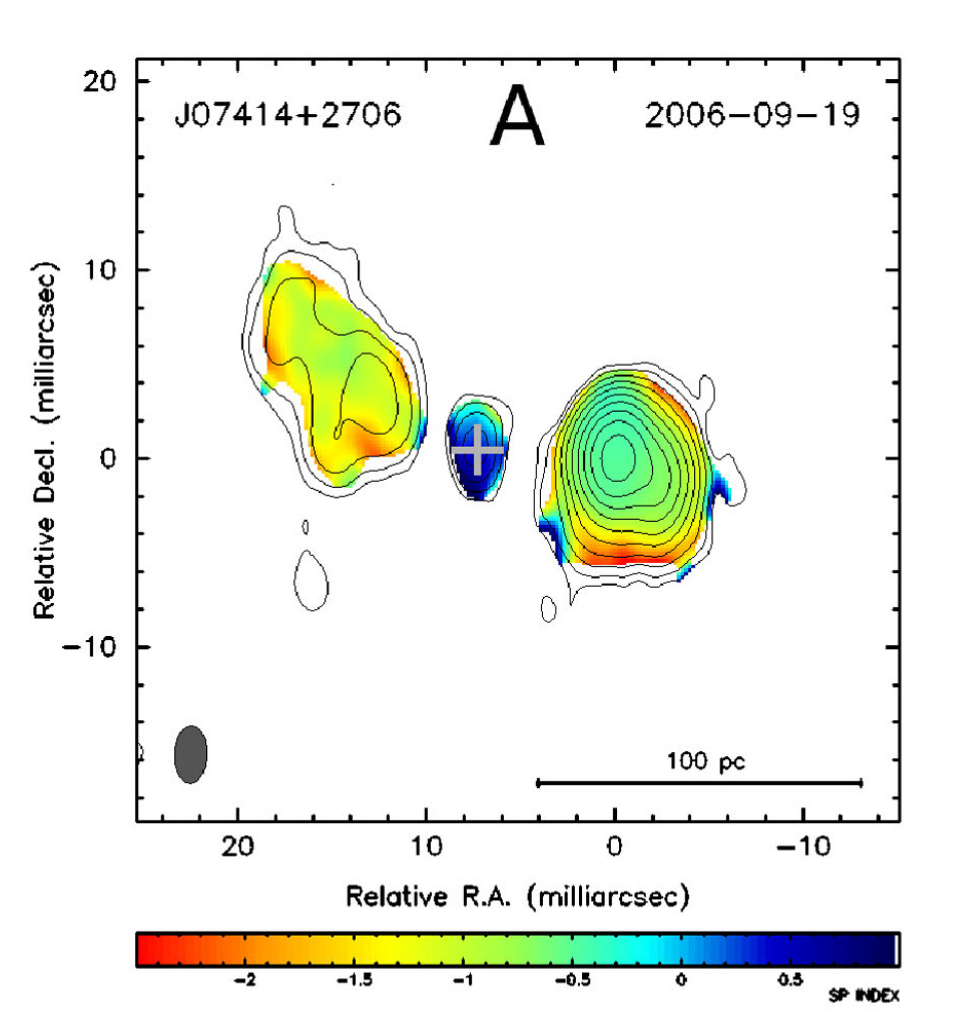
\includegraphics[width=.5\textwidth]{C:/Users/henri/OneDrive/Documents/NTNU/Semester 10/Masteroppgave/Plots/J0741+2706.png}
    \caption{The radio structure of CSO J0741+2706. The core is determined from the flat spectrum component and the symmetry of the radio lobes. Image taken from \cite{Tremblay_2016}}
    \label{fig:CSO_J0741}
\end{figure}

The last two criteria are the newest additions made by \cite{kiehlmann2023compact} and are the best way of separating CSOs from other jetted AGNs. The low variability and lack of relativistic beaming have always been key features of CSOs, but since they were not included in the original classification there have been misidentifications. An example of a source that was previously determined to be a CSO quoted in \cite{kiehlmann2023compact} is the source PKS 1543+005 which shows strong variability and additionally the jet is projected on both sides of the core, giving the illusion of a compact double. With these new criteria, we can be more certain that the sources in the catalogue are similar enough in nature to be able to make more general statements about them.






%\subsection*{Total energy density}
%The total energy density of the photon fields as a function of distance is then seen in figure \ref{fig:photon_fields}. Here one can see that the energy density of the photon fields is constant until the observer is outside the size of the respective regions. From the image it is clear that the biggest contributor to the total energy density becomes the IR torus, but all the regions contribute significantly to the total energy density.

%\subsection*{Spectral energy density}
%The spectral energy density of the different regions is of more interest since this is what will determine the effect of pion decay on protons accelerate in the jet or in the lobes. To create the 
%SED one has estimated the dynamical scale of our system and used the total photon densities to scale the SED accordingly. The resulting SED is seen in figure \ref{fig:SED_sep}. The SED are determined also on a number of 
%parameters, all which have taken from the literature. They are seen in table \ref{tab:SED_params}.

%The choice of variables comes from three sources. \cite{bronzini2024investigating} and \cite{kiehlmann2023compact} which both gives the disk luminosity of CSOs sources, and which we set to $10^{43} erg/s$. \cite{Ghisellini_2009} gives the rest of parameters that relate the different regions to the disk luminosity. The biggest caveat here is that these parameters are not specific to CSOs, but to Blazars in which they are based. For the purposes of this analysis one assumes that the parameters are the same for CSOs as for Blazars, and that one would not expect any significant difference. 







\section{Sub Classification of CSO}
Looking further into the classification of CSOs one now realizes that there are two types of CSOs: CSO 2 and CSO 1. In CSO 2 sources, one considers it edge-brightened where there is significant luminosity in the radio lobes compared to the core. In CSO 1 sources, one considers it edge-dimmed where the luminosity of the radio lobes is significantly lower than that of the core. The origin of the two types of CSOs is thought to be the same, where CSO 1s represent failed CSO 2s. We will get back to the origin later in the report.

The fact of the matter is that the CSO 2 class can further be subdivided. This extra subdivision into CSO 2.0, 2.1, and 2.2 is based on its morphology. The number of Compact Symmetric Objects which succeed into becoming CSO 2s will go through different phases, all with different characteristics. In figure \ref{fig:CSO_2_morphology} we can visualize the different phases of CSO 2 sources. The phases can analogously be compared to the different phases of shock evolution in supernovae.

\begin{figure}
    \centering
    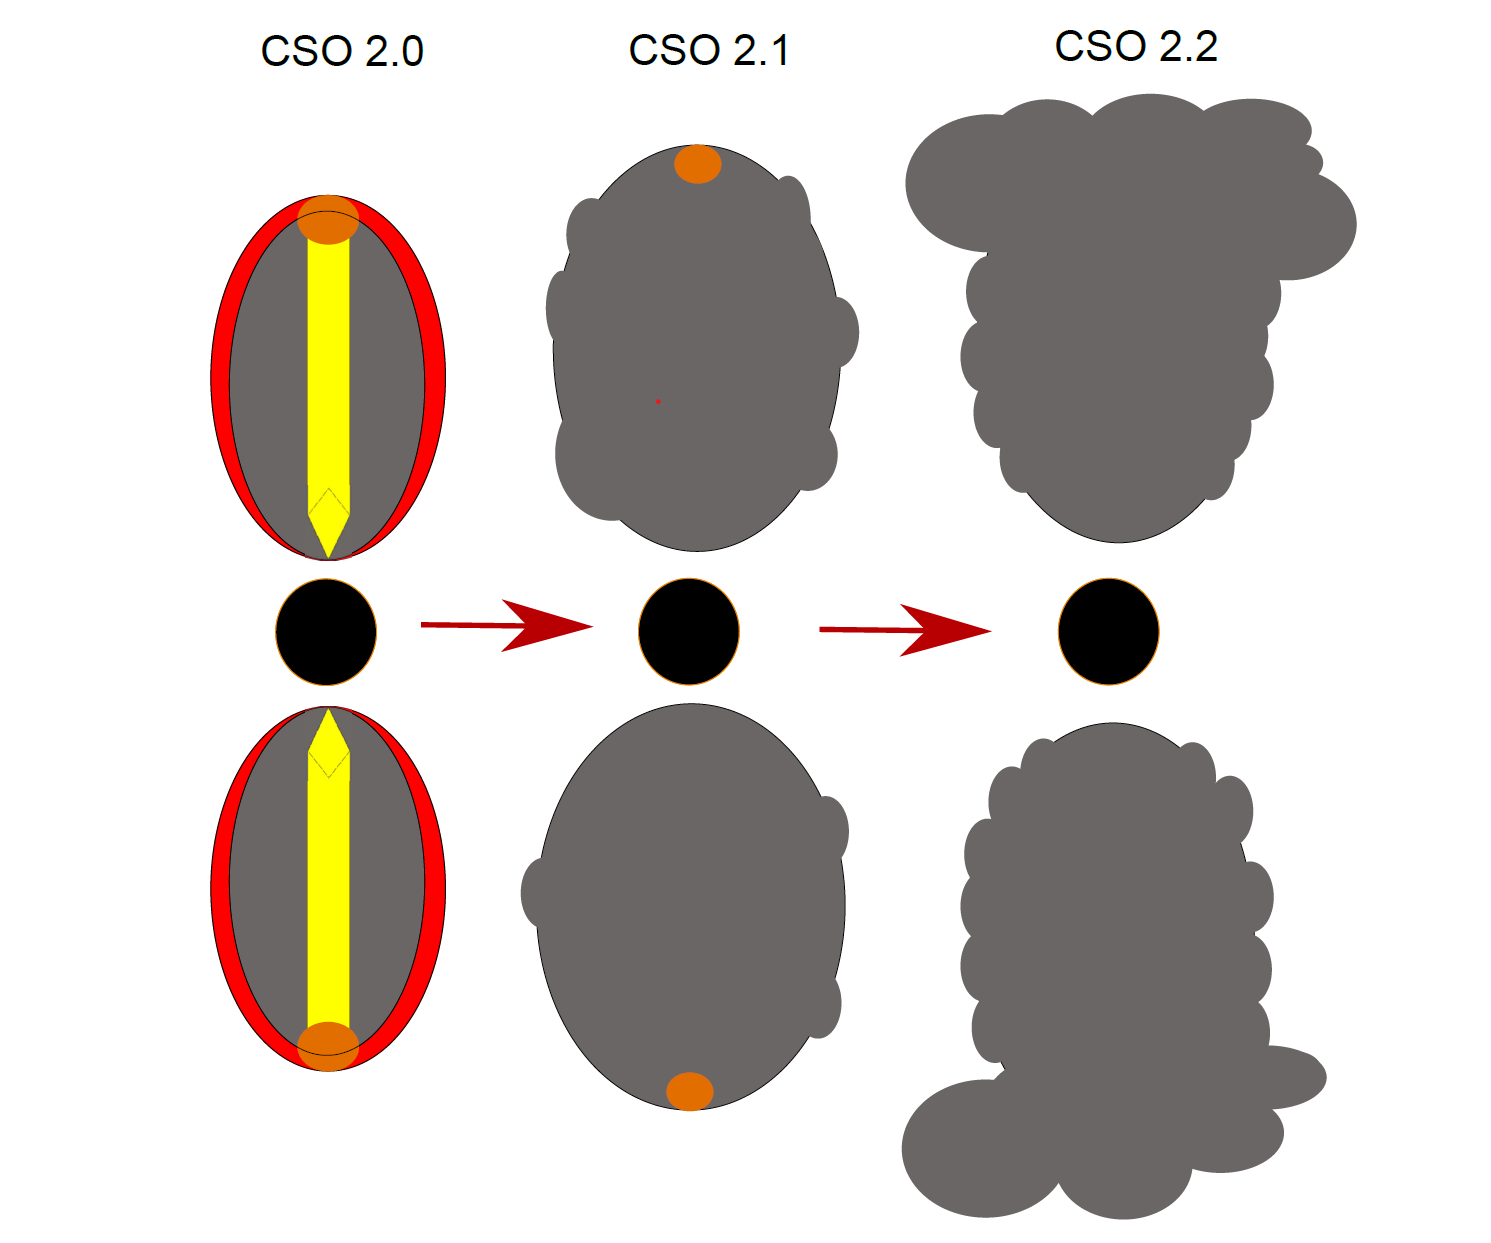
\includegraphics[width=.6\textwidth]{C:/Users/henri/OneDrive/Documents/NTNU/Semester 10/Masteroppgave/Plots/CSO_morphology.png}
    \caption{The different phases of CSO 2 sources. Image taken from \cite{sullivan2024smallscale}}
    \label{fig:CSO_2_morphology}
\end{figure}

\textbf{CSO 2.0}: According to \cite{sullivan2024smallscale}, the CSO 2.0 phase evolves analogously to FRII radio galaxies. The edge-brightened lobes which contain prominent hot spots are similar to typical features of a relativistic jet pushing into the ambient medium. Classical jet models entail the jet collides with the ambient medium and forms two shock fronts, the forward shock and the reverse shock. From shock models, the jet power $L_j$ is what determines the velocity of the forward shock, and in \cite{sullivan2024smallscale} the shock model used gives values similar to observations of CSO 2.0 lobe velocity ($v_c = 0.2c$) and Mach number of approximately $200$.

\textbf{CSO 2.1}: The mid-life or CSO 2.1 is the transition of semi-relativistic jet propagation into the sonic or subsonic regime. The category is often hard to define and is often contaminated by a mix of CSO 2.0 and CSO 2.2. Nevertheless, it remains a separate category since there is still power in the hotspots and the lobes continue to expand but decelerate. 

\textbf{CSO 2.2}: The late life of CSOs or CSO 2.2 is the phase where the jet has decelerated to transonic speeds and the lobes are no longer expanding vertically as a result of jet pressure. The lobes are still expanding due to convectively rising turbulent plumes. When the plumes and the ambient densities are equal, the lobes will stop expanding vertically and start expanding horizontally. %\cite{sullivan2024smallscale} compares it to the characteristic mushroom cloud of volcanic which in this author's opinion paints a very nice image. 

This separation of CSOs will become important since certain environments are more favorable for the production of UHECRs and neutrinos. The most promising candidates are CSO 2.0 sources since they have the highest jet power and the highest velocity of the lobes, which creates a shock front capable of accelerating particles. 

\section{Origin of CSOs/Fueling}
According to \cite{readhead2023compact}, a possible method of igniting these objects is through tidal disruption events. Due to their short lifetime continued discrete ignition events become a good candidate for their birth. Energetically we would assume that we need a massive star to be able to fuel the CSO 2 jets, but it is argued in \cite{sullivan2024smallscale} that this might not be the only solution. They argue that smaller mass stars which encounter the black hole could have sufficient magnetic flux to ignite the extraction of the black hole's angular momentum. The method proposed in \cite{Blandford_1977} relates the extraction of black hole angular momentum to the jet power via 

\begin{equation}
    L_j = \frac{1}{6\pi c} \Omega_{BH}^2 \Phi_{BH}^2
\end{equation}

After the TDE we expect the magnetic flux to disperse around the BH as $\Phi_{BH} \approx \Phi_{\star} \left(\frac{R_{H}}{R_{p}}\right)^2$ where $R_{H}$ is the black hole horizon and $R_{p}$ is the pericenter radius of the stellar encounter. In addition, the magnetic field could be amplified via strong dipolar dynamo action or magneto-rotational instability. The magnetic field could be strong enough to match the jet powers we observe in CSOs today even though the original stellar mass was low. The caveat here is that amplification of the magnetic field is required to reach sufficient levels.


Along with the energetics one can put simple tests on this hypothesis by looking at the fallback time of debris onto a central black hole. This is also done in \cite{sullivan2024smallscale} which quotes the fallback time as 

\begin{equation}
    t_f = 0.5 \text{yr}\left(\frac{M_{\rm BH}}{10^8 M_{\odot}}\right)^{1/2}\left(\frac{M_\star}{M_{\odot}}\right)^{-1}\left(\frac{R_\star}{R_{\odot}}\right)^{3/2}
\end{equation}

For the TDE hypothesis to be correct one would expect the fallback time to be of the order of the lifetime of the CSO 2.0, which is $t_f \approx 1000$ years. From the equation above red giants become a good candidate as they have a large radius and a low mass, and with an SMBH of $10^8 M_{\odot}$ the fallback time is of the order of $1000$ years, a mangnitude equal to that of the predicted lifetime of CSO $2.0$.

For our analysis of CSOs as UHECR sources, the origin of the sources is not of great importance, and we can rely more on observations of the sources. The fact that CSOs harbor a semi relativistic jet is enough to make them viable candidates for UHECRs and neutrinos, something which is observed. Where the TDE hypothesis becomes important is in the understanding of the lifetime of the sources, which relates the eventual density of these sources.


\section{Catalogue of Bona fide CSO}
With the new criteria for CSOs, \cite{kiehlmann2023compact} began compiling a bona fide list of Compact Symmetric Objects. This new catalogue will serve as the testing grounds for their ability to produce UHECRs and neutrinos. The catalogue is a list of 79 sources which are somewhat split between the four different subclasses as seen in table \ref{tab:CSO_class}, where only the CSOs with a spectroscopic redshift have been given a class. The full source catalogue is listed in table \ref{tab:CSO_sources} in the appendix.

The vetting process done in \cite{kiehlmann2023compact} is thorough, and the extended list of what they call A class candidates includes an additional 167 sources which have a high likelihood of being CSOs. In addition to this, they have a list of 1164 B class candidates which are sources that have a lower likelihood of being CSOs, and therefore require a large follow-up study to confirm. The vetting process rejected 1765 sources which were claimed to be CSOs or CSO candidates in other sources and catalogues created since the 1990s. This then creates a great starting block for further investigation, and with the introduction of more sources, more extensive catalogues and luminosity functions can be created. 

%In order to study these sources there will always be a need for observational data. This fact combined with the fact that CSOs are a somewhat new class of AGN mean that there are no large catalogues of pure CSOs, and that many other catalogues misnomer sources as CSOs. This chapter will rely heavily on \cite{kiehlmann2023compact} in which this is discussed and where they define a bona fide catalogue of 79 CSOs. The catalogue will allow us as it has in this paper to say more concrete information about the sources we are studying.

\begin{table}
    \caption{Classification of CSOs in the catalogue.}
    \label{tab:CSO_class}
    \centering
    \begin{tabular}{@{}ccc@{}}
        \toprule
        Class & Number of sources & Percentage of total  \\ \midrule
        CSO 1 & 11 & 14.0  \\
        CSO 2.0 & 17 & 21.5  \\
        CSO 2.1 & 15 & 19.0  \\
        CSO 2.2 & 11 & 14.0  \\
        No class & 25 & 31.6  \\
        \bottomrule
    \end{tabular}
\end{table}
\newpage


\section{Characteristics of CSOs}
Given the new criteria and the new catalogue we can start to peel away the characteristics of CSOs. In figure \ref{fig:redshift_hist} we see the spread of our bona fide CSOs across redshift. The immediate observation is that the majority of CSO 1 sources are in close vicinity. Additionally, the majority of CSO 2.1 and 2.2 are also in closer vicinity compared to CSO 2.0. This distribution is expected since we assume we are observing the higher end of the luminosity function of CSOs, and therefore the most luminous sources will be the ones that are observed at higher redshifts. This figure is complemented by \ref{fig:Luminosity_redshift} where we see a shift to higher luminosity as we move to higher redshifts. This is most likley an observation bias in the sampling of CSOs and that for the most part we are observing the most luminous sources. With the introduction of telescopes with lower flux limit we would assume that the redshift distribution would be more uniform. 

\begin{figure}
    \centering
    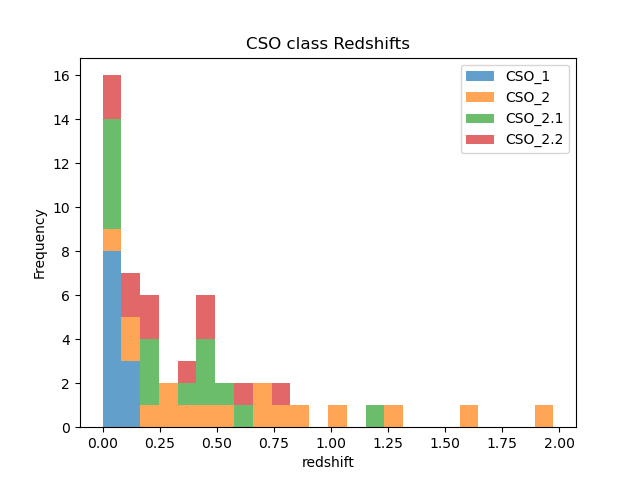
\includegraphics[width=.8\textwidth]{C:/Users/henri/OneDrive/Documents/NTNU/Semester 10/Masteroppgave/Plots/hist_z.png}
    \caption{Distribution of redshift of different classes}
    \label{fig:redshift_hist}
\end{figure}

%We can complement this observation in figure \ref{fig:Luminosity_redshift} where one sees the radio luminosity at peak frequency of CSOs as a function of redshift. Here there is a clear trend toward lower luminosity as we move to lower redshifts. This helps to confirm the observation bias of the redshift distribution. One has also put a line at $z=0.017$ which is the redshift cutoff of $50 Mpc$, the distance which is a limit for the GZK horizon. 

In figure \ref{fig:Luminosity_size} we see the relation between linear size and luminosity at spectral peak. This relation is important since it will give us an idea of the energy deposited into the lobes. The figure shows a clear relation between linear size and emissivity in radio. This relation is expected since the amount of energy deposited into the lobes will affect the size of the lobes. CSO 1 occupy their own region in the plot, giving foundation to the distinction between CSO 1 and CSO 2. The figure does not show a clear distinction between CSO 2.0, 2.1, and 2.2, but one can see that the most luminous sources are CSO 2.0 for a given linear size. 





\begin{figure}
    \centering
    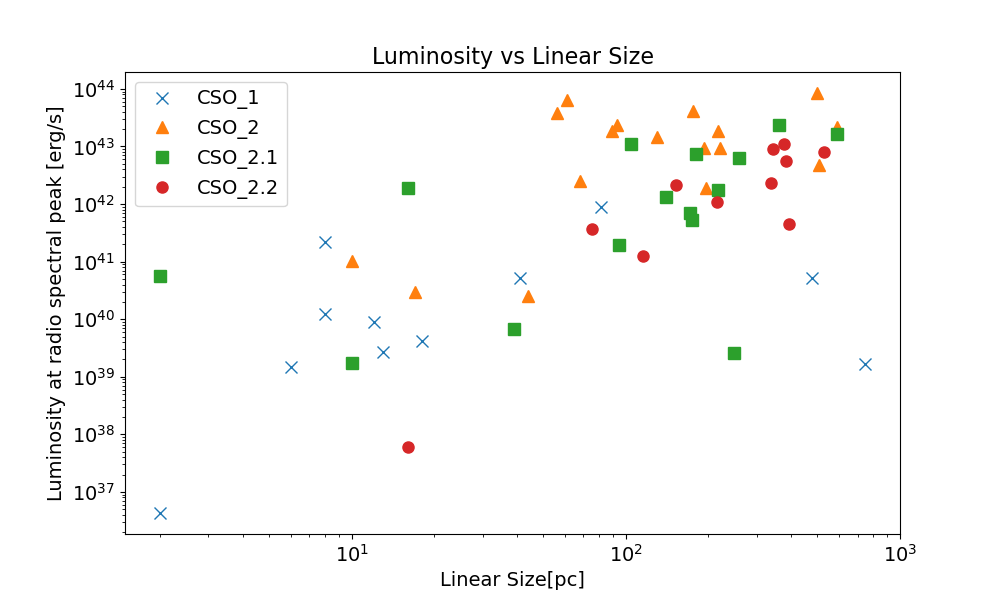
\includegraphics[width=.9\textwidth]{C:/Users/henri/OneDrive/Documents/NTNU/Semester 10/Masteroppgave/Plots/Lin_size_vs_Luminosity.png}
    \caption{The radio luminosity at peak frequency of CSOs as a function of linear size.}
    \label{fig:Luminosity_size}
\end{figure}
\begin{figure}
    \centering
    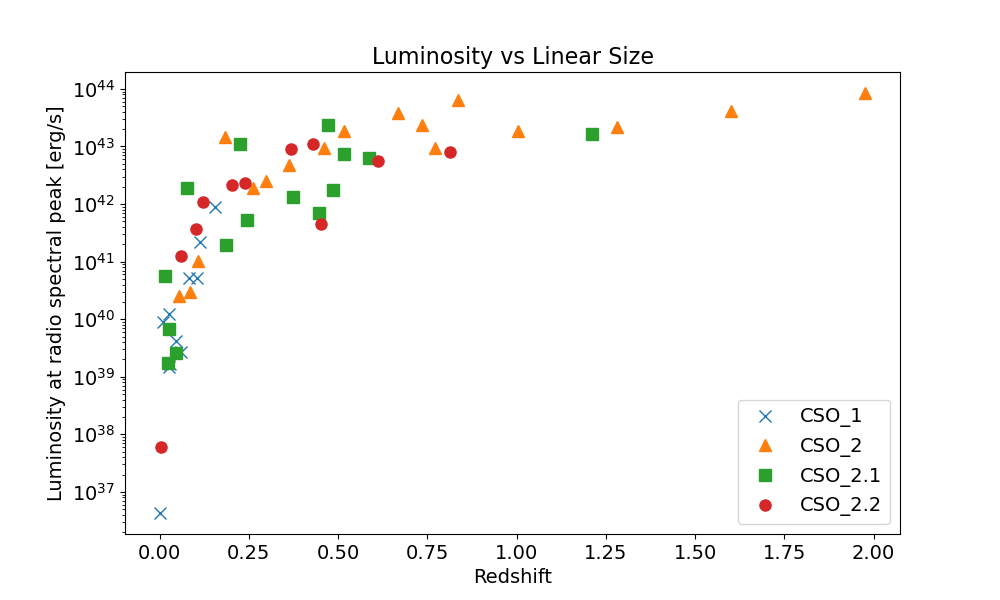
\includegraphics[width=.9\textwidth]{C:/Users/henri/OneDrive/Documents/NTNU/Semester 10/Masteroppgave/Plots/z_vs_Luminosity.png}
    \caption{The radio luminosity at peak frequency of CSOs as a function of redshift.}
    \label{fig:Luminosity_redshift}
\end{figure}

\section{Prevalence of CSOs}
\label{sec:prevalence}

The number density of CSOs is a key factor in determining their viability as UHECR sources. The number density of CSOs is not well known, and the luminosity function of these sources is not defined. Therefore, we can only make a lower limit to their prevalence. From section 4 we defined a method using the lifetime of our objects where the lifetime of CSOs is of the order of $5 \times 10^3$ years. By estimating at which redshift we find an appreciable amount of sources, we can then estimate the number density of these sources.
 In our analysis and follwing \cite{kiehlmann2023compact2} the redshift at which we finds an appreciable amount of sources, is at redshift $z=0.9$. The required number density of these sources to view one source at present time is therefore $1.2 \times 10^{4} \text{Gpc}^{-3} = 1.2 \times 10^{-5} \text{Mpc}^{-3}$. This is a lower limit since we view more than one CSO at present time. 
%The number density of the order of $10^{-5} \text{Mpc}^{-3}$ does not meet the required density of $10^{-4} \text{Mpc}^{-3}$ for UHECRs, but since this is a lower limit for the high luminosity sources, one then requires a bigger part of the luminosity function to be able to produce UHECRs as well.
The number density is within the bounds found in section \ref{sec:prevalence_of_sources}. 

The number density of CSO of $1.2 \times 10^{-5}$ Mpc$^{-3}$ is a reasoable start given the new criteria explained in this section. It remains to see how this number will evolve, and it is clear that any increase in their density will increase their potential as significant UHECRs emitters. The density of CSO marks the biggest change in the discussion surrounding them, where the new criteria have allowed for a much higher density to be estimated. The previous thought that CSOs were young radio galaxies lead to the conclusion in papers such as \cite{TAKAMI2011749} that the density of CSOs is of the order of $10^{-10}$ Mpc$^{-3}$. This is a significant difference, and it is clear that the revival and the new criteria for CSOs as transient objects has allowed for a much higher density to be estimated. We cannot say for certain that the density of CSOs is $1.2 \times 10^{-5}$ Mpc$^{-3}$, but we are very interested in seeing how this number will evolve as more data is collected.







%\section{Stability in jet expansion and lobes.} The most promesing feature of CSOs which we will see as a key feature in the section on time-scales is the stability of the lobes in radio emission, the stability of the jet expansion and the stability of most wavelengths in emissions. In \cite{bronzini2024investigating} they report no significant variablilty of one CSO source in gamma rays, variability of the order of years in x-ray, with the broadband SED showing variability on the timescales of years. This is a clear distincsion from other jetted AGN which are known to be highly variable. Having stable systems allows for more efficient acceleration of ions, and significantly increases the possibility of producing UHECRs. 